\documentclass{article}
\usepackage[french]{babel}
%\usepackage[T1]{fontenc}
\usepackage[utf8]{inputenc}
\usepackage{graphicx} % Required for inserting images
\usepackage{listingsutf8}
\lstset{%
    inputencoding=utf8,
    literate=
        {é}{{\'e}}{1}%
        {è}{{\`e}}{1}%
        {à}{{\`a}}{1}%
        {â}{{\^a}}{1}%
        {ç}{{\c{c}}}{1}%
        {œ}{{\oe}}{1}%
        {ù}{{\`u}}{1}%
        {É}{{\'E}}{1}%
        {È}{{\`E}}{1}%
        {À}{{\`A}}{1}%
        {Ç}{{\c{C}}}{1}%
        {Œ}{{\OE}}{1}%
        {Ê}{{\^E}}{1}%
        {ê}{{\^e}}{1}%
        {î}{{\^i}}{1}%
        {ï}{{\"i}}{1}%
        {ô}{{\^o}}{1}%
        {û}{{\^u}}{1}%
}
\usepackage{fullpage}
\usepackage{setspace}
\usepackage{todonotes}
\usepackage{amsthm}
\usepackage{amsmath}
\usepackage{amssymb}
\usepackage[all]{xy}

\usepackage[french, frenchkw, boxed, linesnumbered]{algorithm2e}

\newtheoremstyle{exostyle}% style name
{10pt}% above space
{10pt}% below space
{}% body font
{}% indent amount
{\scshape\bfseries\large}% head font
{\hfill\vspace{5pt}\newline}% post head punctuation
{0pt}% Space after theorem head
{\hfill\thmname{#1}\thmnumber{ #2} -- \thmnote{ #3}}% head spec

\newtheoremstyle{partiestyle}% style name
{1em}% above space
{1em}% below space
{}% body font
{}% indent amount
{\bfseries}% head font
{\vspace{.5em}\newline}% post head punctuation
{0em}% Space after theorem head
{\thmnumber{#2} \thmnote{ #3}}% head spec

\newtheoremstyle{questionstyle}% style name
{.5em}% above space
{.5em}% below space
{}% body font
{}% indent amount
{\bfseries}% head font
{}% post head punctuation
{0em}% Space after theorem head
{Question \thmnumber{#2 }}% head spec

\theoremstyle{exostyle}
\newtheorem{exo}{Exercice}

\theoremstyle{partiestyle}
\newtheorem{partie}{}[exo]

\theoremstyle{questionstyle}
\newtheorem{question}{Question}[exo]
\newtheorem{questionpartie}{Question}[partie]

\title{Devoir Surveillé Algorithmie Avancée}
\author{L3 MPCI}
\date{8 octobre 2025 - Durée: 1h30}

\begin{document}

\maketitle

\begin{center}
{\em\bf Lorsque l'on vous demande d'écrire de décrire ou de donner un algorithme cela signifiera toujours en donner un pseudo-code, justifier de son exactitude et de sa complexité}

~\\

{\em On rappelle qu'aucun document ni équipement électrique ou électronique n'est autorisé. }
\end{center}


\paragraph*{Les exercices :}
\begin{itemize}
\item sont au nombre de 3;
\item sont indépendants;
\item abordent des sujets différents;
\item sont également jolis et intéressants 
\end{itemize}

\clearpage

\begin{exo}[Tournois]
Un tournoi est un graphe orienté tel que pour  tout couple de sommets $\{x, y\}$, soit $xy$ soit $yx$ est un arc mais pas les deux.

\begin{partie}[Introduction]
	\begin{questionpartie}
		Dessinez un tournoi à 5 sommets.
	\end{questionpartie}
	\begin{questionpartie}
		Combien d'arêtes possède un tournoi à $n$ sommets ?
	\end{questionpartie}
	\begin{questionpartie}
		Combien y a-t-il de tournois à $n$ sommets ?
	\end{questionpartie}
	\begin{questionpartie}
		Montrez que tout tournoi possède un chemin hamiltonien (c'est du cours).
	\end{questionpartie}
	\begin{questionpartie}
		En déduire un algorithme récursif dont vous donnerez la complexité pour trouver un chemin hamiltonien dans un tournoi.
	\end{questionpartie}
\end{partie}
\begin{partie}[méthode probabiliste]
	\begin{questionpartie}
		Montrer que si l'on prend un tournoi à $n$ sommet dont on a tiré l'orientation de chaque arc de façon uniforme et indépendante, la probabilité qu'un chemin hamiltonien donné existe est de $1/2^{n-1}$.
	\end{questionpartie}
	\begin{questionpartie}
		En utilisant la question précédente montrer qu'il existe des tournois à $n$ sommets avec plus de $n!/2^{n-1}$ chemins hamiltoniens différents.
	\end{questionpartie}
	\begin{questionpartie}
		Donnez-en un exemple pour $5$ sommets. 
	\end{questionpartie}
\end{partie}

\begin{partie}[transitivité]
	Un tournoi $T = (V, E)$ est transitif si pour tout triplet $\{x, y, z\}$ de sommets : si $xy$ et $yz$ sont des arcs alors $xz$ aussi.
	\begin{questionpartie}
		Montrez qu'un tournoi transitif ne possède qu'un seul chemin hamiltonien.
	\end{questionpartie}
	\begin{questionpartie}
		Montrer que si pour un chemin hamiltonien $x_1\dots x_n$ d'un tournoi non transitif il existe un arc $x_nx_i$ ou un arc $x_ix_1$, alors il existe (au moins) un deuxième chemin hamiltonien.
	\end{questionpartie}
	\begin{questionpartie}
		Montrer que si $x_1\dots x_n$ est un chemin hamiltonien d'un tournoi non transitif mais que l'on est pas dans le cas de la question précédente il existe un arc :
		\begin{itemize}
			\item $x_jx_i$ avec $1< i < j < n$ tel que pour tout $i'< i < j < j'$ $x_{i'}x_{j'}$ est un arc,
			\item $x_ux_v$ avec $1< i < u < j < v \leq n$ tel que pour tout $ u < u' < i < j < v$ $x_{v'}x_{u'}$ est un arc.
		\end{itemize}
	\end{questionpartie}
	\begin{questionpartie}
		Montrer que si on est dans le cas de la question précédente il existe (au moins) un deuxième chemin hamiltonien.
	\end{questionpartie}
	\begin{questionpartie}
		En déduire qu'un tournoi ne possède un seul chemin hamiltonien que si et seulement si il est transitif.
	\end{questionpartie}

\end{partie}

% https://www.renyi.hu/~p_erdos/1963-08.pdf
% \begin{partie}[Borne inférieure]
% 	Un tournoi $T = (V, E)$ est transitif si pour tout triplet de sommets, si $xy$ et $yz$ sont des arcs alors $xz$ aussi.
% 	\begin{questionpartie}
% 		Soient $v_1, \dots, v_p$ $p$ sommets d'un tournoi $T$ à $n$ sommets. Montrez que si pour tous $1\leq i < j < k \leq p$ $v_iv_j$ est un arc si et seulement si $v_iv_k$ est un arc, alors la restriction de $T$ aux sommets $v_1, \dots, v_p$ est un tournoi transitif.
% 	\end{questionpartie}
% 	\begin{questionpartie}
% 		Donnez un algorithme récursif permettant de construire récursivement une suite $v_1, \dots, v_p$ de $p$ sommets en choisissant à chaque étape un sommet parmi un ensemble $V_i$ que vous déterminerez ($V_1 = V$) de telle sorte que la restriction de $T$ aux sommets $v_1, \dots, v_p$ est un tournoi transitif.
% 	\end{questionpartie}
% 	\begin{questionpartie}
% 		En déduire que l'on peut extraire de tout tournoi à $n$ sommets un tournoi un sous-tournoi avec au minimum $1+\log_2(n)$ sommets.
% 	\end{questionpartie}
	
% \end{partie}

\end{exo}

\clearpage

\begin{exo}[Isomorphisme d'arbres]
	Si $T=(V, E)$ et $T'=(V', E')$ sont deux arbres, un isomorphisme entre $T$ et $T'$ est une bijection $\sigma : V \rightarrow V'$ telle que $xy \in E$ si et seulement si $\sigma(x)\sigma(y) \in E'$. Un automorphisme est un isomorphisme entre $T$ et lui même.
	\begin{partie}[arbres de Cayley]
	~\\

	\begin{figure}[h!]
		\vspace{1cm}
		\begin{center}
			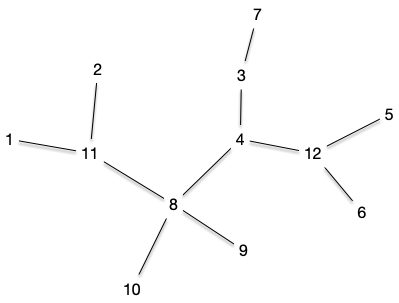
\includegraphics[scale=.4]{arbre-cayley.png}
		\end{center}
		\caption{Un arbre de Cayley.\label{fig-cayley}}
	\end{figure}
	\begin{questionpartie}
		Donnez un automorphisme de l'arbre de la figure~\ref{fig-cayley} qui ne soit pas l'identité.\label{auto-cayley}
	\end{questionpartie}

	\begin{questionpartie}
		Montrez que pour tout isomorphisme d'arbre $\sigma$ entre $T$ et $T'$, si $x$ est une feuille de $T$ alors $\sigma(x)$ est une feuille de $T'$.
	\end{questionpartie}
	\begin{questionpartie}
		En déduire (vous pourrez utiliser la question précédente et effeuiller) que pour tout automorphisme $\sigma$ d'un arbre, il existe soit :
			\begin{itemize}
				\item un sommet invariant $x$ tel que $x = \sigma(x)$,
				\item une arête invariante $xy$ telle que $y = \sigma(x)$ et $x = \sigma(y)$.
			\end{itemize}
	\end{questionpartie}
	\begin{questionpartie}
		Donnez (en le justifiant) le sommet ou l'arête invariante pour tout automorphisme de l'arbre de la figure~\ref{fig-cayley}
	\end{questionpartie}
	\begin{questionpartie}
		Donnez la définition d'un arbre de Cayley planté. Pourquoi est-ce différent d'un arbre planaire ?
	\end{questionpartie}

\end{partie}

\begin{partie}[encodage d'arbres planaires]
	On considère l'encodage récursif $E(T)$ d'un arbre planaire suivant :

	\begin{itemize}
		\item si l'arbre $T$ est réduit à un sommet alors $E(T) = []$
		\item sinon $E(T) = [E(T') \text{pour chaque enfant de T dans l'ordre}]$ 
	\end{itemize}
	~\\

	Chaque sommet est associé à une liste dont les éléments sont les encodage de ses enfants dans l'ordre de parcours.
 Par exemple l'encodage de l'arbre planaire gauche de la figure~\ref{arbres-planaires} est $[\: [], [\: [], []\:]\:]$

	\begin{figure}[h!]
		\vspace{1cm}
		\begin{center}
			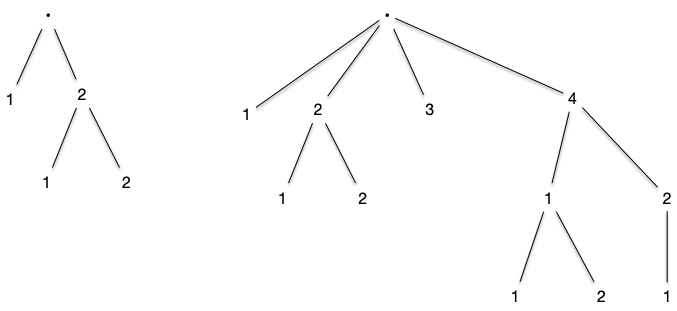
\includegraphics[scale=.4]{arbres-planaires.png}
		\end{center}
		\caption{Deux arbres planaires.\label{arbres-planaires}}
	\end{figure}
	\begin{questionpartie}
		Donnez l'encodage de l'arbre de droite de la figure~\ref{arbres-planaires}.
	\end{questionpartie}
	\begin{questionpartie}
		Donner un algorithme linéaire permettant de rendre l'encodage d'un arbre planaire.
	\end{questionpartie}
	\begin{questionpartie}
		Quelle est la somme des tailles des listes imbriquées encodant un arbre planaire ?
	\end{questionpartie}

\end{partie}
	\begin{partie}[Arbres planaires isomorphes]
	\begin{questionpartie}
		Montrez que tous les automorphismes d'un arbre planté correspondent à des ordres différents des listes de l'encodage de l'arbre.
	\end{questionpartie}
	\begin{questionpartie}
		Donnez tous les automorphismes de l'arbre planaire de gauche de la figure~\ref{arbres-planaires}.
	\end{questionpartie}
	\begin{questionpartie}
		Combien d'automorphismes différents possède l'arbre planaire de droite de la figure~\ref{arbres-planaires} ?
	\end{questionpartie}

	\begin{questionpartie}
		Montrer que deux arbres planaires sont isomorphes si et seulement si le tri de leurs encodages est identique (en utilisant par exemple le tri des listes (possiblement imbriquées) de python).
	\end{questionpartie}

	\begin{questionpartie}
		En déduire un algorithme dont vous donnerez la complexité permettant de savoir si deux arbres planaires sont isomorphes.
	\end{questionpartie}
	\end{partie}
	\begin{partie}[Arbres de Cayley isomorphes]
	\begin{questionpartie}
		Déduire des questions précédentes un algorithme permettant de savoir si deux arbres de Cayley sont isomorphes.
	\end{questionpartie}
	\begin{questionpartie}
		Appliquez votre algorithme à l'arbre de Cayley de la figure~\ref{fig-cayley} et à son arbre isomorphe que vous avez donné question~\ref{auto-cayley}
	\end{questionpartie}

	\end{partie}
	
\end{exo}

\clearpage

\begin{exo}[Coloration (et planarité)]
	On considère le problème suivant :

	\begin{itemize}
		\item {\bf Nom :} 3-Col
		\item {\bf Entrée :} un graphe
		\item {\bf Question :} le graphe en entrée est-il 3 colorable ?
	\end{itemize}
~\\
	On sait que le problème 3-Col est NP-complet.
	\begin{partie}[cours]
		\begin{questionpartie}
			Rappelez définition d'une k-coloration d'un graphe.
		\end{questionpartie}
		\begin{questionpartie}
			Montrer que 3-Col $\leq$ 4-col
		\end{questionpartie}
	\end{partie}

	\begin{partie}[Une 3 coloration particulière]
~\\
\vspace*{-2cm}
		\begin{figure}[h!]
			\vspace{1cm}
			\begin{center}
				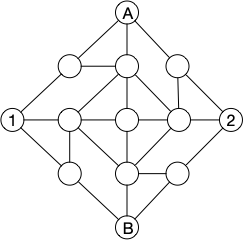
\includegraphics[scale=.4]{gadget-3-col.png}
			\end{center}
			\caption{Un graphe 3 colorable.\label{fig-gadget}}
		\end{figure}
		
		\begin{questionpartie}
			Montrez que le graphe de la figure~\ref{fig-gadget} est 3 colorable.
		\end{questionpartie}
		\begin{questionpartie}
			Donnez une 3-coloration du graphe de la figure~\ref{fig-gadget}.
		\end{questionpartie}
		\begin{questionpartie}
			Montrez que tout 3-coloration du graphe de la figure~\ref{fig-gadget} est telle que :
			\begin{itemize}
				\item la couleur de A est la même que la couleur de B,
				\item la couleur de 1 est la même que la couleur de 2.
			\end{itemize}
		\end{questionpartie}
		\begin{questionpartie}
			Montrez que fixer les couleurs des sommets A et 1 est suffit pour déterminer une 3-coloration du graphe de la figure~\ref{fig-gadget}.
		\end{questionpartie}
	\end{partie}
	\begin{partie}[Une 3 coloration planaire]
	On considère le problème suivant :

	\begin{itemize}
		\item {\bf Nom :} 3-Col-planaire
		\item {\bf Entrée :} un graphe planaire
		\item {\bf Question :} le graphe en entrée est-il 3 colorable ?
	\end{itemize}
		\begin{questionpartie}
			Donnez une définition d'un graphe planaire
		\end{questionpartie}
		\begin{questionpartie}
			Déduire des parties précédentes que le problème 3-Col-planaire est NP-complet (vous pourrez utiliser le graphe 3-colorable pour transformer un dessin non planaire de $G$ en un dessin planaire).
		\end{questionpartie}
		\end{partie}
		\addtocounter{question}{3}
		\begin{question}
			On sait que tout graphe planaire est 4-colorable. Donnez un argument qui montre qu'il est très improbable qu'il existe un algorithme polynomial pour 4-colorer un graphe planaire.
		\end{question}

	
\end{exo}

\end{document}
